\documentclass[english]{article}

%% Packages pull in extra commands:
%% http://en.wikibooks.org/wiki/LaTeX/Packages

\usepackage{hyperref}
\usepackage[latin9]{inputenc}
\usepackage[letterpaper]{geometry}
\geometry{verbose,tmargin=1in,bmargin=1in,lmargin=1in,rmargin=1in}
\usepackage{amsmath}
\usepackage{amssymb}
\usepackage{graphicx}
\usepackage{float}
\usepackage{array}
\usepackage{tikz}
\usepackage{enumerate}
\usepackage{booktabs}
\usepackage{tabularx}
\usepackage{caption} 
\captionsetup[table]{skip=10pt}
\usepackage{authblk}

% New commands serve as shorthand for frequently used command combinations.
\newcommand{\ind}[1]{\mathbf{1}\left(#1\right)}
\newcommand{\bx}{\mathbf{x}}
\newcommand{\E}{\mathbf{E}}

\title{CIS 520, Machine Learning, Fall 2018: Assignment 1}
\author{Shubhankar Patankar}

\begin{document}
\maketitle

{\normalsize \noindent Collaborators:  \underline{}}


\section{Conditional independence in probability models}

\begin{enumerate} 
\item $p(x_i) = \sum_{j = 1}^{k} f_j(x_i) \pi_{j}$ 

\item The formula for $p(x_1, \dots, x_n)$ can be derived as follows:
\\Assuming $x_1, \dots, x_n$ are independent,
$$p(x_1, \dots, x_n) =\prod_{m = 1}^{n} p(x_m)$$ 
$$\therefore p(x_1, \dots, x_n) = \prod_{m = 1}^{n} \bigg(\sum_{j = 1}^{k} f_j(x_m) \pi_{j}\bigg)$$

\item The formula for $p(z_u = v \mid x_1, \dots, x_n)$ can be derived as follows:  
\\ It is known that $p(x_u  \mid z_u = v) = f_v(x_u)$. Therefore, the probability of the $u$-th data point $p(x_u)$ can be uniquely determined given the knowledge that it is generated by function $v$. Similarly, the probability that the $u$-th data point is generated by the $v$-th function is dependent solely on the knowledge of the data point $x_u$ itself, not the entire data set. 
$$\therefore p(z_u = v \mid x_1, \dots, x_n) = p(z_u = v \mid x_u)$$
Using Bayes Rule, 
$$p(z_u = v \mid x_u) = \frac{p(x_u \mid z_u = v) p(z_u = v)}{p(x_u)}$$
$$\therefore p(z_u = v \mid x_u) = \frac{f_v(x_u) \pi_{v}}{\sum_{j = 1}^{k} f_j(x_u) \pi_{j}}$$ \\ \\
Alternatively,
$$p(z_u = v \mid x_1, \dots, x_n) = \frac{p(x_1, \dots, x_n \mid z_u = v) p(z_u = v)}{p(x_1, \dots, x_n)}$$
$$p(z_u = v \mid x_1, \dots, x_n) =  \frac{p(x_u \mid z_u = v) p(z_u = v) \bigg[\prod_{i = 1, i \neq u }^{n} \bigg(\sum_{j = 1}^{k} f_j(x_i) \pi_{j}\bigg)\bigg]}  {\sum_{j = 1}^{k} f_j(x_u) \pi_{j}  \bigg[\prod_{i = 1, i \neq u }^{n} \bigg(\sum_{j = 1}^{k} f_j(x_i) \pi_{j}\bigg)\bigg]}$$
$$\therefore p(z_u = v \mid x_u) = \frac{f_v(x_u) \pi_{v}}{\sum_{j = 1}^{k} f_j(x_u) \pi_{j}}$$ 
\end{enumerate}

\section{Non-Normal Norms}

\begin{enumerate}
\item

For the given vectors,the point closest to $x_1$ under each of the following norms is \\\\
$\lVert x_1 - x_2 \rVert = [0.1, -0.6, -0.3, -0.4]$ \\
$\lVert x_1 - x_3 \rVert = [0.2, -0.9, 0.1, 0]$ \\
$\lVert x_1 - x_4 \rVert = [0, 2.6, 0, 0.9]$ \\ \\

a) $L_0$: $x_4$ with distance = $2$ \\
b) $L_1$:  $x_3$ with distance =  $1.2$\\
c) $L_2$: $x_2$ with distance = $0.787$ \\
d) $L_{\inf}$: $x_2$ with distance =  $0.6$\\

\item 
Draw the 1-Nearest Neighbor decision boundaries with the given norms and lightly shade the o region: In all figures below, blue refers to 'x' and yellow to 'o'. For the L-0 norm, most of the space is unclassifiable with the exception of the lines marked. Points (4,1) and (5,4) are not classifiable. The code used to generate decision boundaries for norms $L_1$, $L_2$ and $L_{\inf}$ is included in the Appendix. \\ \\ a) $L_0$ \qquad \qquad \qquad \qquad \qquad \qquad \qquad \qquad b) $L_1$\\ 
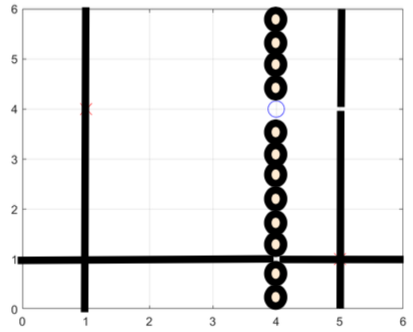
\includegraphics[width=0.35\textwidth]{L_0.png}
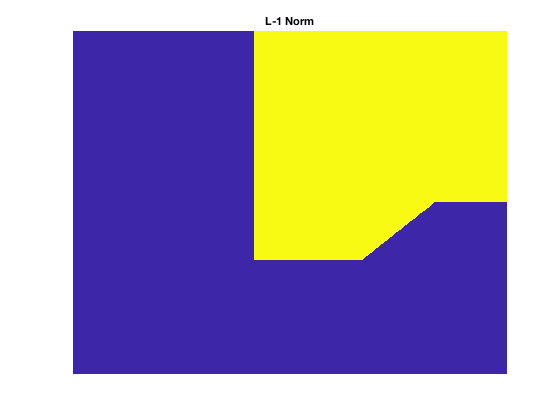
\includegraphics[width=0.4\textwidth]{L_1.png} \\
c) $L_2$ \qquad \qquad \qquad \qquad \qquad \qquad \qquad \qquad d) $L_{\inf}$\\
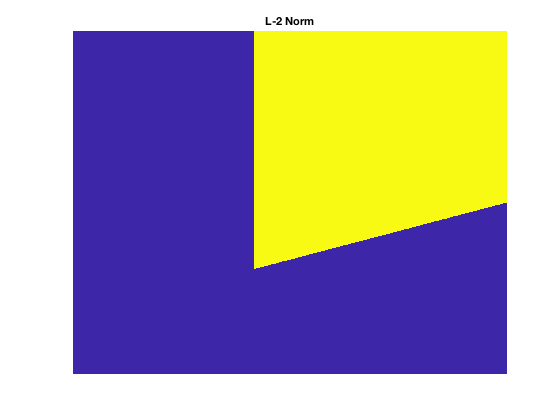
\includegraphics[width=0.4\textwidth]{L_2.png}
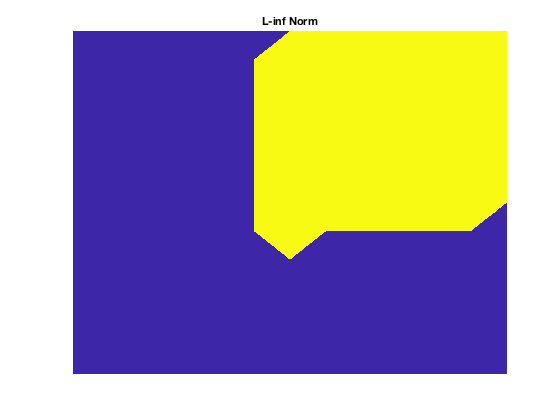
\includegraphics[width=0.4\textwidth]{L_inf.png} \\

\end{enumerate}

\pagebreak
\section{Decision trees}
\subsection{Part 1}
The sample entropy $H(Y)$ can be written as:
$$H(Y) = -P(Y = +) \log_{2} (P(Y = +)) - P(Y = -) \log_{2} (P(Y = -))$$
$$\therefore H(Y) = (16/30) \log_{2} (16/30) - (14/30) \log_{2} (14/30) = 0.9968$$
The information gains are given by $IG(X_i) = H(Y) - H(Y \mid X_i)$.

\begin{align*}
  \therefore H(Y \mid X_1) =&\; P(X_1 = T) \bigg[-P(Y = + \mid X_1 = T) \log_{2} (-P(Y = + \mid X_1 = T)) \\
  -&\; P(Y = - \mid X_1 = T) \log_{2} (-P(Y = - \mid X_1 = T))\bigg] \\
  +&\; P(X_1 = F) \bigg[-P(Y = + \mid X_1 = F) \log_{2} (-P(Y = + \mid X_1 = F)) \\
  -&\; P(Y = - \mid X_1 = F) \log_{2} (-P(Y = - \mid X_1 = F))\bigg] \\
  =&\; (13/30)\bigg[(-6/13) \log_{2}(6/13) - (7/13) \log_{2}(7/13) \bigg] \\
  +&\; (17/30)\bigg[(-10/17) \log_{2}(10/17) - (7/17) \log_{2}(7/17) \bigg] \\
  =&\; 0.9852
\end{align*}

$$\therefore IG(X_1) = 0.9968 - 0.9852 = 0.0115$$

\begin{align*}
  H(Y \mid X_2) =&\; P(X_2 = T) \bigg[-P(Y = + \mid X_2 = T) \log_{2} (-P(Y = + \mid X_2 = T)) \\
  -&\; P(Y = - \mid X_2 = T) \log_{2} (-P(Y = - \mid X_2 = T))\bigg] \\
  +&\; P(X_2 = F) \bigg[-P(Y = + \mid X_2 = F) \log_{2} (-P(Y = + \mid X_2 = F)) \\
  -&\; P(Y = - \mid X_2 = F) \log_{2} (-P(Y = - \mid X_2 = F))\bigg] \\
  =&\; (11/30)\bigg[(-4/11) \log_{2}(4/11) - (7/11) \log_{2}(7/11) \bigg] \\
  +&\; (19/30)\bigg[(-12/19) \log_{2}(12/19) - (7/19) \log_{2}(7/19) \bigg] \\
  =&\; 0.9480
\end{align*}

$$\therefore IG(X_2) = 0.9968 - 0.9480 = 0.0488$$

\begin{figure}[H]
\centering
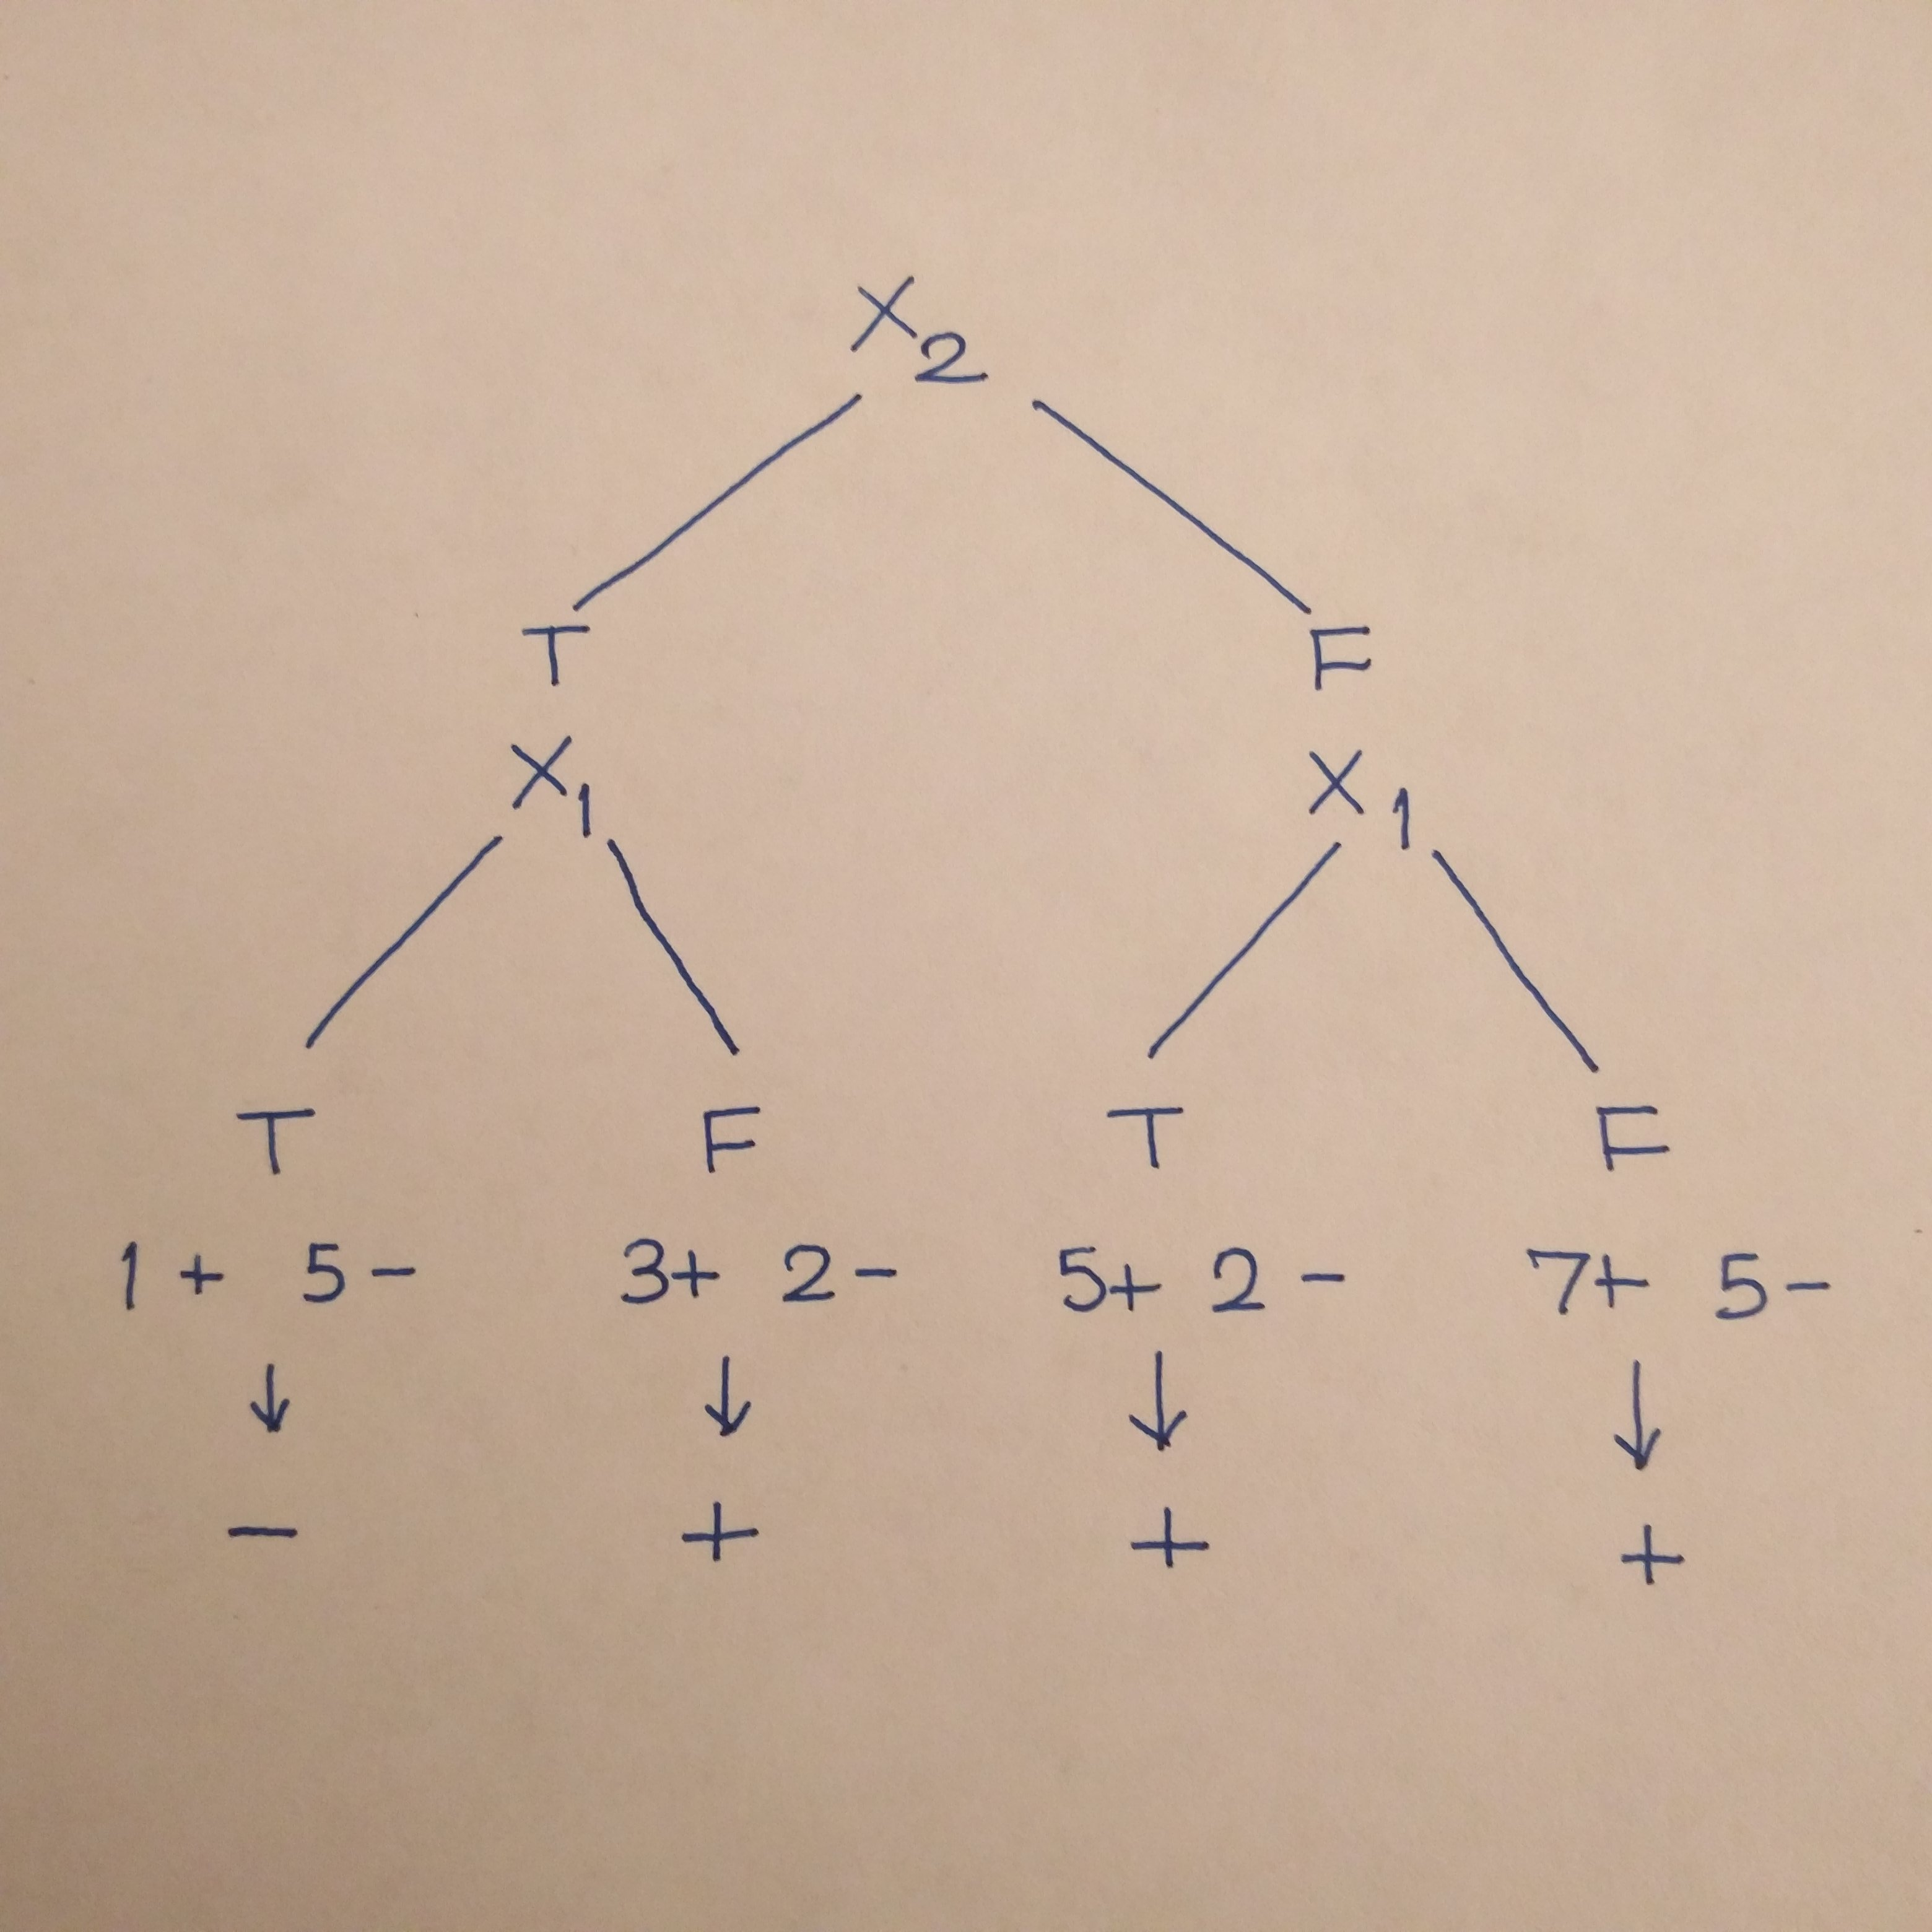
\includegraphics[scale = 0.075]{DT}
\caption{Decision Tree}
\label{fig:DT}
\end{figure}

\subsection{Part 2}
\begin{enumerate}
	\item If variables X and Y are independent, is $IG(x,y) = 0$? If yes, prove it. If no, give a counter example.
	$$X\perp Y \implies p(x,y) = p(x)p(y)$$
	\begin{align*}
	\therefore IG(x,y) =& -\sum_{x} \sum_{y} p(x,y) \log{\bigg(\frac{p(x)p(y)}{p(x,y)}\bigg)} \\
	=& -\sum_{x} \sum_{y} p(x,y) \log{\bigg(\frac{p(x)p(y)}{p(x)p(y)}\bigg)} \\
	=& -\sum_{x} \sum_{y} p(x,y) \log{(1)} = 0 \\
	\end{align*}
	\pagebreak
	\item Proof that $IG(x,y) = H[x] - H[x \mid y] = H[y] - H[y \mid x]$,
	starting from the definition in terms of KL-divergence:
	\begin{align*}
	IG(x,y) =&\; KL\left(p(x,y)||p(x)p(y)\right) \\
	=&\;  -\sum_{x} \sum_{y} p(x,y) \log{\bigg(\frac{p(x)p(y)}{p(x,y)}\bigg)} \\
	=&\; -\sum_{x} \sum_{y} p(x,y) \big[\log{p(x)} + \log{p(y)} - \log{p(x,y)}\big] \\
	=&\; -\sum_{x} \sum_{y} \big[p(x,y)\log{p(x)} + p(x,y)\log{p(y)} - p(x,y)\log{p(x,y)}\big] \\
	=&\; -\sum_{x} \sum_{y} p(x,y)\log{p(x)} -\sum_{x} \sum_{y} p(x,y)\log{p(y)} + \sum_{x} \sum_{y} p(x,y)\log{p(x,y)} \\
	=&\; -\sum_{x}  p(x)\log{p(x)} - \sum_{y} p(y)\log{p(y)} + \sum_{x} \sum_{y} p(x,y)\log{p(x,y)} \\
	=&\; H[x] + H[y] - H[x,y] \\
	=&\; H[x] + H[y] - (H[y \mid x] + H[x]) \\
	=&\; H[y] - H[y \mid x] \\
	=&\; H[x] - H[x \mid y] \\
	\end{align*}
\end{enumerate}

\section{High dimensional hi-jinx}

\begin{enumerate}
\item Intra-class distance.
  \begin{align*}
    \E[(X - X')^2] =&\; \E[X^2 - 2XX' + X'^2] \\
    =&\; \E[X^2] - 2\E[XX'] +\E[X'^2] \\
    =&\; \E[X^2] - 2\E[X]\E[X'] +\E[X'^2] \\
     =&\; ({\mu_1}^2 + \sigma^2) - 2{\mu_1}^2 + ({\mu_1}^2 + \sigma^2) \\
     =&\; 2\sigma^2
  \end{align*}

\item Inter-class distance.
  \begin{align*}
    \E[(X - X')^2] =&\; \E[X^2 - 2XX' + X'^2] \\
    =&\; \E[X^2] - 2\E[XX'] +\E[X'^2] \\
    =&\; \E[X^2] - 2\E[X]\E[X'] +\E[X'^2] \\
     =&\; ({\mu_1}^2 + \sigma^2) - 2{\mu_1}{\mu_2} + ({\mu_2}^2 + \sigma^2) \\
     =&\; {\mu_1}^2 - 2{\mu_1}{\mu_2} + {\mu_2}^2 + 2\sigma^2 \\
     =&\; (\mu_1 - \mu_2)^2 + 2\sigma^2
  \end{align*}

\item Intra-class distance, m-dimensions.
  \begin{align*}
    \E\bigg[\sum_{j=1}^m (X_{j} - X'_{j})^2\bigg] =&\; \E\bigg[\sum_{j=1}^m\big({X_{j}}^2 - 2X_{j}X'_{j} + {X'_{j}}^2\big)\bigg] \\
    =&\; \E\bigg[\sum_{j=1}^m {X_{j}}^2\bigg] - 2\E\bigg[\sum_{j=1}^m X_{j}X'_{j}\bigg] + \E\bigg[\sum_{j=1}^m {X'_{j}}^2\bigg] \\
    =&\; \sum_{j=1}^m\E\big[ {X_{j}}^2\big] - 2\sum_{j=1}^m\E\big[ X_{j}X'_{j}\big] + \sum_{j=1}^m\E\big[ {X'_{j}}^2\big] \\
    =&\; \sum_{j=1}^m\E\big[ {X_{j}}^2\big] - 2\sum_{j=1}^m\E\big[ X_{j}\big]\E\big[X'_{j}\big] + \sum_{j=1}^m\E\big[ {X'_{j}}^2\big] \\
    =&\; \sum_{j=1}^m({\mu_{1j}}^2 + \sigma^2) - 2\sum_{j=1}^m {\mu_{1j}}^2 + \sum_{j=1}^m({\mu_{1j}}^2 + \sigma^2) \\
    =&\; m\sigma^2 +  m\sigma^2 = 2m\sigma^2 \\
  \end{align*}

\item Inter-class distance, m-dimensions.
  \begin{align*}
    \E\bigg[\sum_{j=1}^m (X_{j} - X'_{j})^2\bigg] =&\; \E\bigg[\sum_{j=1}^m\big({X_{j}}^2 - 2X_{j}X'_{j} + {X'_{j}}^2\big)\bigg] \\
    =&\; \E\bigg[\sum_{j=1}^m {X_{j}}^2\bigg] - 2\E\bigg[\sum_{j=1}^m X_{j}X'_{j}\bigg] + \E\bigg[\sum_{j=1}^m {X'_{j}}^2\bigg] \\
    =&\; \sum_{j=1}^m\E\big[ {X_{j}}^2\big] - 2\sum_{j=1}^m\E\big[ X_{j}X'_{j}\big] + \sum_{j=1}^m\E\big[ {X'_{j}}^2\big] \\
    =&\; \sum_{j=1}^m\E\big[ {X_{j}}^2\big] - 2\sum_{j=1}^m\E\big[ X_{j}\big]\E\big[X'_{j}\big] + \sum_{j=1}^m\E\big[ {X'_{j}}^2\big] \\
    =&\; \sum_{j=1}^m({\mu_{1j}}^2 + \sigma^2) - 2\sum_{j=1}^m {\mu_{1j}}{\mu_{2j}} + \sum_{j=1}^m({\mu_{2j}}^2 + \sigma^2) \\
    =&\; \sum_{j=1}^m {\mu_{1j}}^2 - 2 \sum_{j=1}^m {\mu_{1j}}{\mu_{2j}} + \sum_{j=1}^m {\mu_{2j}}^2 + 2m\sigma^2 \\
  \end{align*}

\item The ratio of expected intra-class distance to inter-class
  distance is: 
  $$ratio = \frac{2m\sigma^2}{\sum_{j=1}^m {\mu_{1j}}^2 - 2 \sum_{j=1}^m {\mu_{1j}}{\mu_{2j}} + \sum_{j=1}^m {\mu_{2j}}^2 + 2m\sigma^2}$$  
  The denominator can be re-written as follows:
  \begin{align*}
    denominator =&\; {\mu_{11}}^2 + \sum_{j=2}^m {\mu_{1j}}^2 - 2 \bigg({\mu_{11}}{\mu_{21}} + \sum_{j=2}^m {\mu_{1j}}{\mu_{1j}}\bigg) + {\mu_{21}}^2 + \sum_{j=2}^m {\mu_{1j}}^2 + 2m\sigma^2 \\
    =&\; {\mu_{11}}^2 - 2{\mu_{11}}{\mu_{21}} + {\mu_{21}}^2  + 2m\sigma^2 \\
     =&\; ({\mu_{11}} - {\mu_{21}})^2 + 2m\sigma^2 \\
  \end{align*}
   $$\therefore ratio = \frac{2m\sigma^2}{({\mu_{11}} - {\mu_{21}})^2 + 2m\sigma^2}$$  
  As $m$ increases towards $\infty$, this
  ratio approaches $1$. This indicates that the extra dimensions do not provide valuable information to help classify $y$ as their number approaches infinity.
\end{enumerate}

\section{Fitting distributions with KL divergence}

KL divergence for Gaussians.

  \begin{enumerate}
  \item The KL divergence between two univariate Gaussians is given as follows:
    \begin{align*}
      KL(p(x) || q(x)) =&\; \E_{p}\bigg[\log\frac{p(x)}{q(x)}\bigg] \\
      =&\; \int_{-\infty}^{\infty} p(x) \log\frac{p(x)}{q(x)} dx \\
      =&\; \int_{-\infty}^{\infty} p(x) \log{p(x)} dx - \int_{-\infty}^{\infty} p(x) \log{q(x)} dx \\
      =&\; \int_{-\infty}^{\infty} p(x)\bigg[\log\bigg(\frac{1}{\sqrt{2 \pi \sigma^2}}\bigg) - \frac{1}{2\sigma^2}(x-{\mu_{1}})^2\bigg] dx \\
      -&\;  \int_{-\infty}^{\infty} p(x)\bigg[\log\bigg(\frac{1}{\sqrt{2 \pi}}\bigg) - \frac{1}{2}(x-{\mu_{2}})^2\bigg] dx \\
      =&\; \int_{-\infty}^{\infty} p(x) \log\bigg(\frac{1}{\sqrt{2 \pi \sigma^2}}\bigg) dx - \int_{-\infty}^{\infty} p(x) \log\bigg(\frac{1}{\sqrt{2 \pi}}\bigg) dx \\
      +&\; \int_{-\infty}^{\infty} p(x) \frac{(x-{\mu_{2}})^2}{2} dx - \int_{-\infty}^{\infty} p(x)\frac{(x-{\mu_{1}})^2}{2\sigma^2} dx \\
      =&\; \log\bigg(\frac{1}{\sqrt{2 \pi \sigma^2}}\bigg) - \log\bigg(\frac{1}{\sqrt{2 \pi}}\bigg) + \int_{-\infty}^{\infty} p(x) \bigg[ \frac{(x-{\mu_{2}})^2}{2} - \frac{(x-{\mu_{1}})^2}{2\sigma^2} \bigg] dx\\
      =&\; \E_{p}\bigg[ \frac{(x-{\mu_{2}})^2}{2} - \frac{(x-{\mu_{1}})^2}{2\sigma^2} \bigg] + \log\bigg(\frac{1}{\sigma}\bigg) \\
      =&\; \mathbf{E}_p[ f(x, \mu_1, \mu_2, \sigma)] + g(\sigma) \\
      =&\; \frac{1}{2} \E_{p}[(x-{\mu_{2}})^2] - \frac{1}{2 \sigma^2} \E_{p}[(x-{\mu_{1}})^2] + \log\bigg(\frac{1}{\sigma}\bigg) \\
      =&\; \frac{\E_p[x^2-2\mu_2x+\mu_2^2]}{2} - \frac{1}{2} + \log\bigg(\frac{1}{\sigma}\bigg) \\
      =&\; \frac{\E_p[x^2]}{2} - \mu_2\E_p[x] + \frac{\mu_2^2}{2} -  \frac{1}{2} + \log\bigg(\frac{1}{\sigma}\bigg) \\
      =&\; \frac{\sigma^2 + \mu_1^2}{2} - \mu_1\mu_2 + \frac{\mu_2^2}{2} - \frac{1}{2} + \log\bigg(\frac{1}{\sigma}\bigg) \\
      \end{align*}
      
  \item The value $\mu_1 = \mu_2$ minimizes $KL(p(x)||q(x))$. This follows from taking the partial derivative with respect to $\mu_1$ of the above result for the KL divergence and setting it to $0$. 
    \begin{align*}
      0 =&\; \frac{\partial KL(p(x) || q(x))}{\partial \mu_1} \\
      0 =&\;  \mu_1 - \mu_2\\
      \mu_1 =&\; \mu_2
    \end{align*}
  \end{enumerate}

\section{Appendix}
Matlab Code for 2.2
\begin{verbatim}
clc; clear; close all;

x = 0:0.001:6;
y = 6:-0.001:0;
[X,Y] = meshgrid(x,y);
D_x_1 = [1,4];
D_x_2 = [5,1];
D_o = [4,4];

p1 = sqrt((abs(X - D_x_1(1))).^2 + (abs(Y - D_x_1(2))).^2);
p2 = sqrt((abs(X - D_x_2(1))).^2 + (abs(Y - D_x_2(2))).^2);
p3 = sqrt((abs(X - D_o(1))).^2 + (abs(Y - D_o(2))).^2);
data(:,:,1) = p1;
data(:,:,2) = p2;
data(:,:,3) = p3;
[~,I] = min(data,[],3);
I(I == 1) = 0;
I(I == 2) = 0;
I(I == 3) = 1;
figure;
imagesc(I);
title('L-2 Norm');
axis off

clc; clearvars -except X Y D_x_1 D_x_2 D_o;

p1 = ((abs(X - D_x_1(1))) + (abs(Y - D_x_1(2))));
p2 = ((abs(X - D_x_2(1))) + (abs(Y - D_x_2(2))));
p3 = ((abs(X - D_o(1))) + (abs(Y - D_o(2))));
data(:,:,1) = p1;
data(:,:,2) = p2;
data(:,:,3) = p3;
[~,I] = min(data,[],3);
I(I == 1) = 0;
I(I == 2) = 0;
I(I == 3) = 1;
figure;
imagesc(I);
title('L-1 Norm');
axis off

clc; clearvars -except X Y D_x_1 D_x_2 D_o;

p1_1 = (abs(X - D_x_1(1)));
p1_2 = (abs(Y - D_x_1(2)));
p1 = max(p1_1, p1_2);
p2_1 = (abs(X - D_x_2(1)));
p2_2 = (abs(Y - D_x_2(2)));
p2 = max(p2_1, p2_2);
p3_1 = (abs(X - D_o(1)));
p3_2 = (abs(Y - D_o(2)));
p3 = max(p3_1, p3_2);
data(:,:,1) = p1;
data(:,:,2) = p2;
data(:,:,3) = p3;
[~,I] = min(data,[],3);
I(I == 1) = 0;
I(I == 2) = 0;
I(I == 3) = 1;
figure;
imagesc(I);
title('L-inf Norm');
axis off

clc; clearvars -except X Y D_x_1 D_x_2 D_o;

p1_temp(:,:,1) = (abs(X - D_x_1(1)));
p1_temp(:,:,2) = (abs(Y - D_x_1(2)));
p1 = sum(p1_temp ~= 0, 3);

p2_temp(:,:,1) = (abs(X - D_x_2(1)));
p2_temp(:,:,2) = (abs(Y - D_x_2(2)));
p2 = sum(p2_temp ~= 0, 3);

p3_temp(:,:,1) = (abs(X - D_o(1)));
p3_temp(:,:,2) = (abs(Y - D_o(2)));
p3 = sum(p3_temp ~= 0, 3);

data(:,:,1) = p1;
data(:,:,2) = p2;
data(:,:,3) = p3;
[~,I] = min(data,[],3);
I(I == 1) = 0;
I(I == 2) = 0;
I(I == 3) = 1;
figure;
imagesc(I);
title('L-0 Pseudo-Norm');
axis off
\end{verbatim}

\end{document}
